%!TEX root = vaisagh_thesis.tex

\chapter{The Building Blocks of a Behavior Model for Egress Simulation}
\label{chapter:IBEVAC}

In the previous chapter, the salient features of the behavior of a crowd engaging in egress were introduced. It is understood that people don't immediately exit a building on hearing a fire alarm or seeing smoke. The occupant gets only an inkling about the danger that is possible. In both these cases there is not enough information for him to get scared and make the decision to egress. If the cues are interesting enough, he then embarks on investigating to gather more information. On realizing that the situation requires some action, he forms a plan to evacuate either alone or, if possible, with his primary group members. In forming this plan of evacuation, unless he is trained for egress or very familiar with the environment, it is unlikely that he will have knowledge of all exits. As a result, he is most likely to just move to the nearest \emph{known} exit. An overview of this process of human evacuation is illustrated in Fig.~\ref{fig:EvacuationProcess}.
% Whatever action they are undertaking, they preserve social norms as far as possible by not shoving or pushing other people~\cite{Cocking:2005uc,Drury:2009ga,Torres:2010tj}.

\begin{figure}[!htb]
\centering
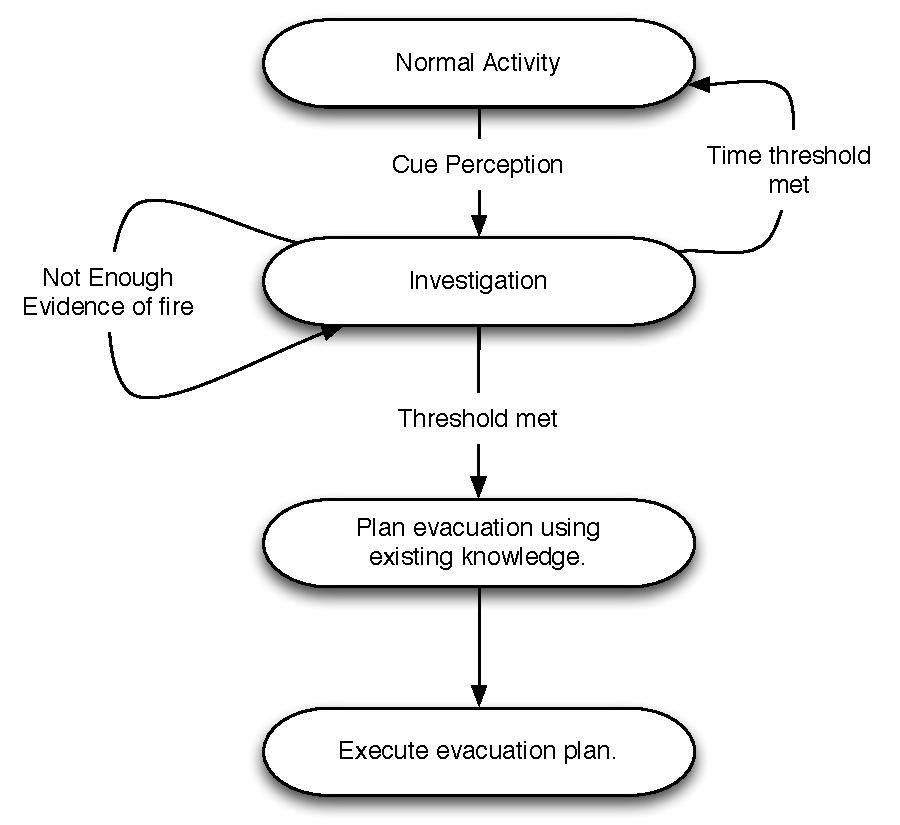
\includegraphics[height=4in]{InfoBasedArchitecture/ProcessOfEvacuation}
\caption[The Process of Evacuation]{The Process of Evacuation: This state diagram shows the different phases of behavior of a person engaging in egress and the triggers that cause phase changes}
\label{fig:EvacuationProcess}
\end{figure}


A small set of core subprocesses and their interaction is necessary and sufficient to produce this evacuation process. These are introduced in Section~\ref{IBEVAC:EgressProgress}. Section~\ref{sec:shortcomings_in_existing_models} introduces some of the shortcomings of existing approaches to modelling each of these sub processes. Section~\ref{IBEVAC:Contributions} explains how these shortcomings are addressed and overviews the key contributions of this thesis.




% section existing_agent_architectures (end)

\section{The Building Blocks of the Egress Process}
\label{IBEVAC:EgressProgress}

The individual behevaior of an evacuee during emergency egress was summarized in Figure~\ref{fig:EvacuationProcess} from the literature discussed in Chapter~\ref{chapter:LiteratureReview}. This section outlines the building blocks of a system that simulates crowd egress during an emergency event. The first step in simulating the behavior of any human being engaging in an activity is modelling his \emph{perception} of the environment. Once perceived, the information gained from perception is used to \emph{identify events} and trigger key actions. In the case of an egress simulation, this would be evacuation (or one of the processes leading up to it). Following this, the person tries to form an evacuation plan using the \emph{knowledge} he has of the layout of the environment and also the information that he is currently perceiving. Once such a plan is formed, a \emph{path is planned} towards this point and he moves along this path towards his goal. Thus the process of egress simulation can be said to consist of four major building blocks: perception, event identification, spatial knowledge utilization and navigation. The following sections defines and explains each of these building blocks and their significance in the evacuation process.

\subsection{Perception}
\label{IBEVAC:IBP}

	Perception refers to the process by which an environment is observed by a person. For an agent, this implies that it should extract features from the environment. These features are called percepts~\cite{Russel:1995vi}. Each percept gives the evacuee certain information about the environment. At the simplest level, percepts provide the agent information about the location and the environment around it and thus allows it move naturally around the environment. In some cases, something out of the ordinary like a ringing fire alarm or smoke or even people running away from a location, might be perceived. Communication between agents can also be considered to be a mode of perception since it is a process by which additional information is gained by the agents. The perception process is the main interface of the agent with the environment through which it gets all the information needed to act. In order to act on information perceived, it is essential for the agent to be able to identify events that require some action.
    % This idea of looking at perception as a process of gathering information is referred to, in this thesis, as \emph{information based perception}.

\subsection{Event identification}
\label{IBEVAC:EventIdentification}

	  In some cases, evacuees might perceive something out of the ordinary like a ringing fire alarm or smoke or even people running away from a location. If these special percepts, known as \emph{cues}, are intriguing enough, then the occupant will set about investigating the environment in search of more cues that would help make a decision on a plan of action. Cues are certain changes in the environment that indicate that something is wrong or different from normal~\cite{Sime:1983uy}. Thus, cues help people identify an event and a need for an action. During emergency egress, on perceiving \emph{sufficient} cues from the environment, an evacuee stops whatever task he's doing and initiates a process of investigation. Once enough evidence is gathered to convince the evacuee of danger, evacuation starts. If enough information is not obtained then the evacuee will likely resume their previous task. Thus identification of events is a key component of the evacuation process that is especially important for modelling pre-evacuation behavior.

    % A person's intrinsic characteristics like age, gender and mental state determine how much information is considered enough i.e.\ the threshold. Each person keeps a track of all the cues that are perceived and when the amount of information crosses the threshold, the evidence is acted upon. In the first phase, this action would be to start investigation and in the second phase it would be the starting of the process of evacuation. In this thesis, this whole process by which the evacuee perceives, analyses and aggregates cues and identifies an event is called \emph{event identification}.

    In summary, event identification is the process by which the evacuee interprets perceived information and decides to proceed to the next phase of evacuation. Executing the action for a particular phase generally requires the evacuee to proceed to a particular location in the environment. This is done using the subjective knowledge that he has of the environment.

\subsection{Spatial knowledge utilization}
\label{IBEVAC:Knowledge}

	On recognizing that there is an event to escape from, the evacuee moves towards the closest known exit. Each evacuee holds his own personal version of the map of the environment which is used for evacuation and movement in general. This personal map is called his cognitive map~\cite{tolman1948}. In most cases, this map is not complete. In a scenario where all known exits are blocked or if the evacuee does not know any exit, he is likely to engage in some sort of exploration behavior which helps increase his knowledge and improve his cognitive map.

    The process of knowledge modelling encompasses the method used for modelling the cognitive map and how it is obtained by the evacuee and his actions when insufficient knowledge is available to act. Modelling evacuee-specific \emph{knowledge} is necessary to model the heterogeneity in behavior found in real life emergency evacuations. The key function of the spatial knowledge model for the agent is to provide it with a target to move to complete the action required based on the event identified. The actual movement towards this point is controlled by the navigation system.


\subsection{Navigation}
\label{IBEVAC:Navigation}

	Navigation is defined as the process or activity of accurately ascertaining one's position and planning and following a route. In the context of egress simulation, we define navigation as the process by which an evacuee first plans his route towards a \emph{goal location} based on his cognitive map and then moves along this route towards the goal. Thus, navigation consists of 2 distinct processes: planning a route and following the route. The former is referred to as path planning and the latter is called motion planning.

    During emergency egress, once evacuation has started, the agent decides that it must proceed to a particular exit, say exit D. Given the current location and this goal, the path planning system recommends a sequence of locations, or waypoints, through which the agent should proceed to get to this goal. Understanding the process of path planning in agent based simulations is easier if it is divided into two parts:  A higher level path finder that finds abstract logical waypoints towards the goal, i.e. go through room A to room B to room C and take Exit D; and a lower level mechanism that translates these logical waypoints to physical locations on the map that the agent can pass through to reach it's goal. Fig.~\ref{fig:detailedNavigationModule}, which gives a mathematical overview of the navigation process, refers to the former as ``Logical Waypoint Determination'' and the latter as ``Current Waypoint Path Determination''. Once these physical waypoints are determined the actual movement towards these locations are determined by the motion planning process.

    Motion planning is a term borrowed from robotics which originally means detailing a task into discrete motions. In the context of crowd simulation, we use the term motion planning to refer to the task of finding a collision free velocity to get from the current point to the next waypoint in the planned path. The motion planning layer ensures that the agent manages to reach its next way point without colliding with other agents.

    Assuming that the cognitive map is modelled as a graph with the edges $E$ representing \emph{areas} or rooms in the environment, Figure~\ref{fig:NavigationArchitecture} gives a mathematical model of how navigation is generally modelled.


    % To explain the working of the navigation module, we make use of the illustration in Fig.~\ref{fig:detailedNavigationModule}.  In this thesis, the cognitive map is implemented as a graph with the edges indicating \emph{areas} or rooms in the environment and $E_i$ refers to an $i^{th}$ edge of the graph in the agent's cognitive map.

    \begin{figure}[!tb]
    \centering
    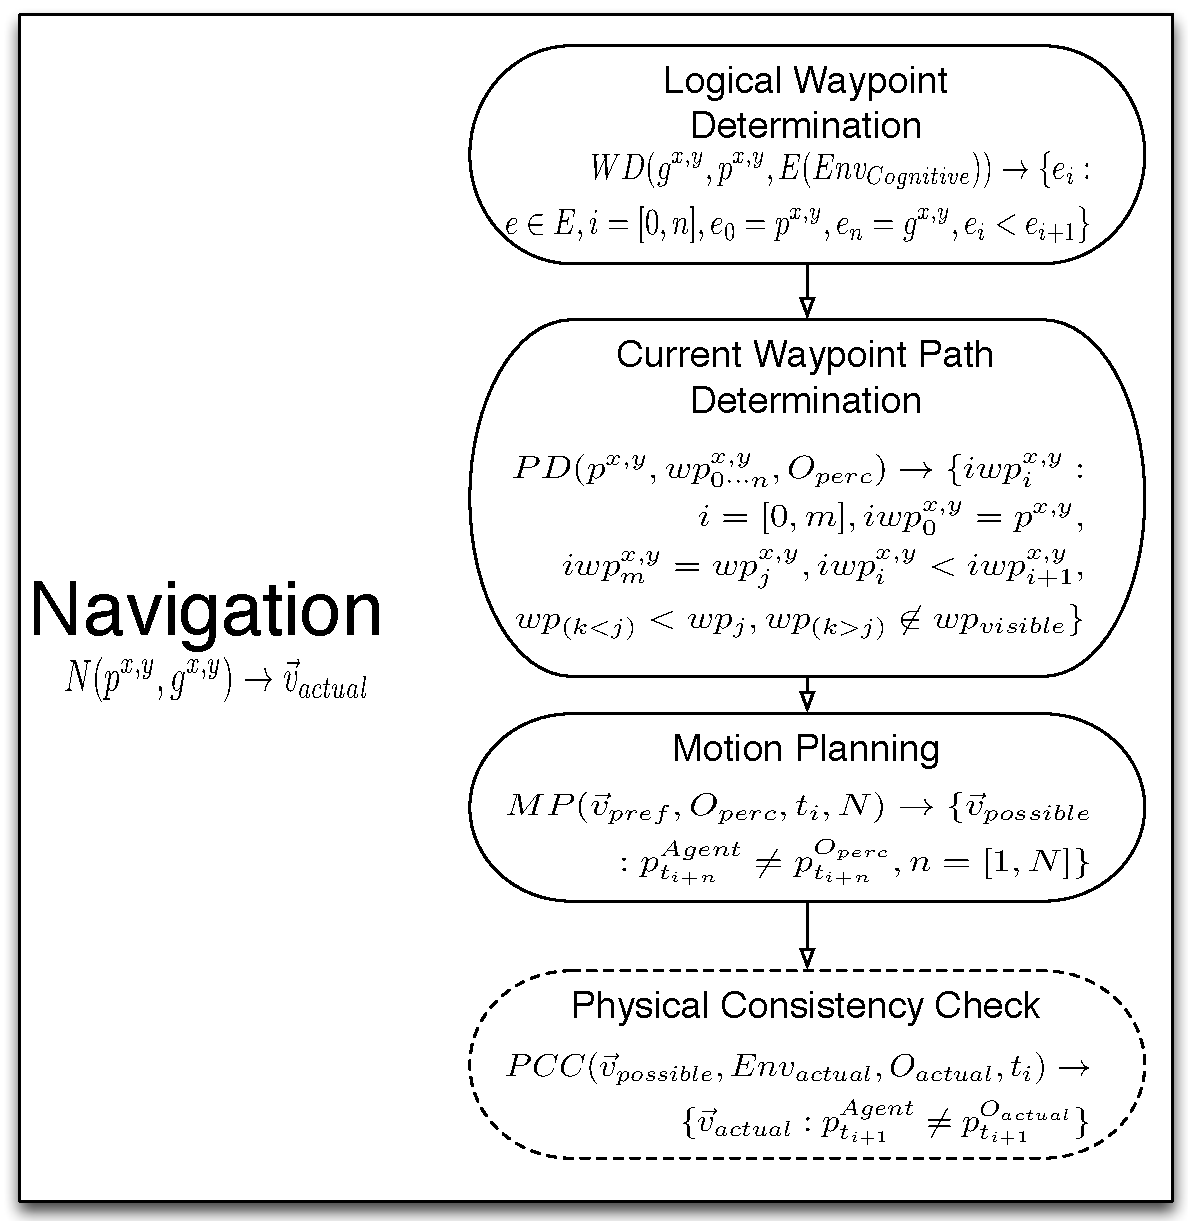
\includegraphics[height=5in]{InfoBasedArchitecture/NavigationWithFormula}
    \caption[Detailed Navigation Model]{Mathematical description of the working of a Navigation System}
    \label{fig:detailedNavigationModule}
    \end{figure}

    The goal position~($g^{x,y}$) is first received by the \emph{Logical Waypoint Determination}~($WD$) system which then uses a route finding algorithm like A-star or Djikstra's to find a set of logical waypoints~($E_i$) that will lead the agent from its current position($p^{x,y}$) to the goal position~($g^{x,y}$). The logical waypoints in the path so planned will be a list of links from the agent's cognitive map~($Env_{cognitive}$). This implies two things: Firstly, it looks at the environment at the room/ area level. Secondly, the agent plans a path according to his personal cognitive map hence there is no garantuee that the path planned by two agents from the same point will be exactly the same. This step is called a waypoint determination step because it returns a set of logical waypoints to be used by the agent to reach its goal. This set of logical waypoints is then passed to the next level of navigation, i.e.\ \emph{the Current Waypoint Path Determination} step.

    The \emph{Current Waypoint Path Determination}~($PD$) differs from the higher layer in that it takes into consideration dynamic obstacles i.e.\ other agents, as well as the static obstacles to determine a collision free path from the current location to the farthest visible waypoint. The logical waypoints are first converted to a set of concrete waypoints~($WP^{x,y}$) which are actual locations on the map. Using the set of perceived obstacles~($O_{perc}$) a set of intermediate waypoints~($IWP^{x,y}$) that would enable a collision free path to the farthest visible concrete waypoint~($wp^{x,y}_j$) is calculated and passed to the next level. This level can also be referred to as the \emph{strategic planning step} since it tries to model how a person strategically moves from one point to another while ensuring that it minimizes collisions with others. Nan's pattern based approach~\cite{Nan:2011vr} and ClearPath by Guy et al.~\cite{Guy:2009gu} are examples of models for this layer.

    The preferred velocity of the agent is then set to the velocity that would lead it to the next intermediate concrete waypoint. Following this, the Motion Planning System like RVO~\cite{Guy:2010ko,Yeh:2008tg} or Social force~\cite{Helbing:1995ie} based methods determine the actual movement of the agent for the next time step of the simulation based on this prefered velocity. At each time step~($t_i$), the motion planning system take a preferred velocity~($\vec{v}_{pref}$) and set of obstacles~($O_{perc}$) (both static and dynamic) as input and outputs a possible velocity~($\vec{v}_{possible}$) that the agent can use to ensure that collisions do not occur for the next $N$ seconds. The two important points of difference from the previous layer is that it has some noticeable effect only when a collision is imminent and that it is very short term (limited to a few time steps) as compared to PD.

    % Since the Motion Planning system works on the basis of perceived obstacles and not actual obstacles, there is a chance, especially in dense environments, that the predicted velocity might cause a collision. In such cases, the lowest level \emph{Physical Consistency Check}~($PCC$) layer ensures that unnatural behavior is not produced. As the name suggests, this layer ensures that physical consistency is maintained and people don't walk through other people and static obstacles in the environment during the next time step~($t_{i+1}$). This is the only layer in the agent that uses the actual map($Env_{actual}$) and actual obstacles($O_{actual}$) instead of the personal cognitive map and perceived obstacles.

    To summarize, the navigation system receives a goal that is passed to the highest level which determines a high level route through the different areas in the environment to the goal; this waypoint is passed to the next level which determines a path towards the current waypoint that avoids dynamic obstacles and calculates the velocity of the agent in order to get to the waypoint while avoiding collisions for the next time step of the simulation.




In summary, a perception system along with event identification, a knowledge model and a navigation system can together be used to produce the entire process of a person evacuating from a building. The function of each of these building blocks is summarized in Table~\ref{tab:BuildingBlocks}. In the following sections, we first identify shortcomings in existing models of these processes and then explain the contributions of this thesis to those areas.

% Requires the booktabs if the memoir class is not being used
\begin{table}[tbp]
\centering
\topcaption{The Building Blocks of Human Behavior during Egress} % requires the topcapt package
\begin{tabular}{p{1.0in}   p{2.1in}   p{2.4in}} % Column formatting, @{} suppresses leading/trailing space
\hline\hline %inserts double horizontal lines
Building Block & Definition & Purpose \\
\hline
Perception  & The process of gathering information about the environment. & Learn about the environment and observe events.\\[3pt]
Event Identification & The process by which the evacuee analyses and aggregates cues and identifies an event.  & Change from one phase to another based on perception and internal state.\\[3pt]
Knowledge Modellings & The process of using stored knowledge to formulate a plan for evacuation. & Determining a goal based on the current spatial cognitive map. \\[3pt]
% Communication & The process of knowledge transfer between evacuees. & Exchange of information between evacuees and management by trained staff. \\[3pt]
Navigation & The routing and movement process. & Handles movement towards the evacuee's current goal. \\[3pt]
% Task Management & Higher level management of strategies and tasks for each phase. & Simplifies the handling of multiple tasks to be completed at each phase of the evacuee's pre-evacuation and evacuation behavior. \\[3pt]
\bottomrule
\end{tabular}
\label{tab:BuildingBlocks}
\end{table}

\section{Shortcomings in Existing Models} % (fold)
\label{sec:shortcomings_in_existing_models}

The previous section identified the core building blocks of an agent based model of emergency egress. In Chapter~\ref{chapter:LiteratureReview}, the salient features of human behavior during egress were identified and summarized in Section~\ref{LiteratureReview:PsychSummary}. In this section, we use this to identify key research questions in each of the core building blocks, where either new modelling approaches or new understanding is necessary.


\subsection{Perception : the lack of a realistic approach}
\label{IBEVAC:PerceptionShortcomings}


    Perception is the process by which agents perceive and gather information about the world around them. It is thus a crucial part of an agent based simulation of crowds. However, in most models, it is standard practice to consider a simple circular or elliptical sensor range. All agents and objects within that sensor range are perceived by the agent. One of the rare exceptions to this is the MASSegress model~\cite{Pan:2006vp} that makes use of a ray tracing algorithm to model perception. The assumptions that an agent can perceive as many objects as are there in the sensor range without any internal limit on capacity~\cite{Miller:1956tr} and that perception is simply a visual process are both simplistic. Another related consequence of the limited information processing capacity of humans is that the human brain tries to chunk similar information to improve it's efficiency. modelling this limited information processing capacity and chunking can produce significant improvements in the realism of crowd simulations. This is demonstrated in Chapter~\ref{chapter:IBP} which introduces an Information Processing Based Perception model which takes this into account.


\subsection{Event identification: modelling pre-evacuation behavior}
\label{IBEVAC:EventIdentificationShortcomings}

    % The Event Knowledge Module stores the agent's beliefs about the current state of the environment.

    Several studies~\cite{Kuligowski:2009un} have shown that humans do not evacuate immediately on hearing a fire alarm. This delay between hearing the alarm and actual evacuation has even resulted in deaths~\cite{Berry:2000us}. This can have significant results on the time to evacuation and the general efficiency of evacuation. However, despite several studies highlighting this, pre-evacuation behavior is hardly ever modeled. In the few instances were it is considered~~\cite{Pires:2005gs,Franca:2009el} , the models are rather simplistic.
    % In essence, there is a need for an agent to keep a track of the phase of evacuatio.
    % Event identification can be considered to be equivalent to the process of associating perceived cues with an experience in a Recognition Primed D.

    Chapter~\ref{chapter:PreEvacuationBehavior} introduces a model for event identification that enables the modelling of pre-evacuation behavior and studying of its effects. Through simulation of certain scenarios, the importance and usefulness of modelling pre-evacuation behavior is demonstrated.


\subsection{Knowledge modelling: the effect of partial knowledge}
\label{IBEVAC:EnvironmentKnowledgeShortcomings}

    On deciding to evacuate an evacuee plans a path towards an exit. Ideally, this plan would be to move towards the closest exit that is known. In most cases, however, say a shopping mall or a hospital, it is highly likely that the majority of the occupants do not know emergency exit locations or the closest exits. How evacuees explore and form their memory in such a situation of partial knowledge is still an open problem.

    Existing simulations either assume complete knowledge or have a simplistic memory model where a single visit is remembered forever. It is unlikely that evacuees have such eidetic memories. Also, it is common to simply take a depth first approach to exploration in case of incomplete knowledge. However, there is no proof whether this is the actual way in which evacuees explore.

    Chapter~\ref{chapter:SpatialKnowledgeChapter} first introduces a game based methodology for studying exploration of indoor environments and how human memory works during exploration. By comparing against a pure random walker, it is shown that humans are in fact more effective explorers than a random walker but not as efficient as is portrayed in existing computational models of egress. The study also revealed some interesting patterns in the strategies used for exploring complex indoor environments.


\subsection{Navigation: analyzing motion planning systems}
\label{IBEVAC:NavigationShortcomings}

    The motion planning system used in an agent based simulation of egress is a key determinant of the kind of behavior produced by the model. The motion planning system used can have a great impact on the patterns of motion produced and the dynamics of the crowd.
    There are several different models of motion planning that have been proposed that sometimes work in very different ways. Each model has its strengths and there are studies that demonstrate their strengths. However, despite the abundance of models, there aren't any standard methods for comparing different models.
    In Chapter~\ref{chapter:MotionPlannerComparison} of this thesis, we quantitatively compare and evaluate existing motion planning systems and determine a metric that can be used for differentiating existing motion planning systems and compare their working against real world data.


% section perception_modelling (end)



% section shortcomings_in_existing_models (end)

\section{Contributions of the Remaining Chapters}
\label{IBEVAC:Contributions}

Following is a summary of the contributions of the remaining chapters:

\begin{itemize}
    \item \textbf{Chapter~\ref{chapter:IBP}:} This chapter presents an Information Processing Based model of perception which was presented at the Cyberworlds 2011 Conference~\cite{Viswanathan:2011uy} and further explored in the extended version published in the Transactions on Computational Science~\cite{Viswanathan:ut}. This chapter additionally contains some validation of the model against real world experimental data.
    \item \textbf{Chapter~\ref{chapter:PreEvacuationBehavior}:} This chapter presents a method for modelling pre-evacuation behavior in emergency egress simulation. The model was presented at the Pedestrian and Evacuation Dynamics Conference in 2012 and published in 2014~\cite{Viswanathan:2012vt}.
    \item \textbf{Chapter~\ref{chapter:SpatialKnowledgeChapter}:} A game based methodology for studying the effect of memory on exploration of complex indoor environments and different exploration strategies used is presented in this chapter. The work done in this chapter has been submitted for review to Nature Scientific Reports.
    \item \textbf{Chapter~\ref{chapter:MotionPlannerComparison}:} The final contribution of this thesis is a methodology for quantitatively comparing different motion planning systems which was also used to compare some popular models against real world data. These findings were published in European Physical Journal B~\cite{Viswanathan2014}.
\end{itemize}


\section{Summary}
\label{IBEVAC:Summary}

% This chapter introduced the IBEVAC Agent Architecture for modelling complex behavior in agent based simulations of crowds. This architecture consists of and \emph{Information Based Perception Module} as a sensor, a \emph{Knowledge Base} consisting of both events and the environment, an \emph{Agent Descriptor Module} which could be used to specify the properties of the agents, a \emph{Planning Module} for planning and a \emph{Navigation Module} and \emph{Communication Module} as actuators. The rest of the thesis develops each of these components to form.

This chapter first summarized the behavior of an evacuee during evacuation from the literature in the previous Chapter. Following this, the four essential building blocks for an agent based simulation of emergency egress was presented. Following this, shortcomings of existing approaches to modelling these parts were identified and the contributions of the remaining chapters was introduced.